\documentclass[11pt,a4paper]{article}

\usepackage[utf8]{inputenc}
\usepackage[T1]{fontenc}
\usepackage{lmodern}
\usepackage[margin=2.3cm]{geometry}
\usepackage{amsmath,amssymb,amsthm}
\usepackage[round,authoryear]{natbib}
\usepackage{xcolor}
\usepackage{hyperref}
\usepackage{enumitem}
\usepackage{graphicx}
\usepackage{booktabs}

\hypersetup{colorlinks=true,linkcolor=blue!60!black,
  citecolor=green!50!black,urlcolor=blue!70!black}

\newcommand{\ee}{\mathrm{e}}
\newcommand{\dd}{\mathrm{d}}
\newcommand{\NN}{\mathbb{N}}
\newcommand{\RR}{\mathbb{R}}
\newcommand{\Ck}{\mathcal{C}}
\newcommand{\phit}{\tilde\phi}

\theoremstyle{plain}
\newtheorem{theorem}{Theorem}
\newtheorem{proposition}[theorem]{Proposition}
\newtheorem{corollary}[theorem]{Corollary}
\newtheorem{lemma}[theorem]{Lemma}
\theoremstyle{remark}
\newtheorem*{remark}{Remark}

\title{A Visual Landscape for Doi--Peliti Reaction-Network Universality\\[4pt]
  \large Placing CRNs on the Puiseux stratification of
  algebraic Dyson--Schwinger equations}
\author{S. Amarteifio\\
  \small\textit{Percolation Labs}}
\date{April 2026}

\begin{document}
\maketitle

\begin{abstract}
When the Doi--Peliti (DP) path integral of a reaction network is
rewritten as a Dyson--Schwinger equation (DSE) for its dressed
propagator, one obtains an equation of the form
$G(z) = z\,\phi(G(z))$ with $\phi$ a polynomial in $G$.  This
places the DP generating function squarely inside the class of
algebraic generating functions studied by analytic combinatorics,
where the coefficient asymptotics
$[z^{n}]G \sim A\,z_{\star}^{-n}\,n^{-\tau}$ are controlled
entirely by the Puiseux exponent of the dominant branch of
$F(G,z) = G - z\phi(G)$.  The Flajolet--Sedgewick transfer
theorem and the Banderier--Drmota dyadic-ceiling result for
positive ($\NN$-algebraic) systems together produce an explicit
landscape whose strata $\Ck_{k}$ carry the exponents
$\tau_{k} = 1 + 1/k$.  We describe this landscape in visual form
for the cubic case; we place the directed-percolation family,
pair coagulation, triplet annihilation and Schlögl~II on it; we
note the specific points where these families intersect a
higher-order stratum; and we observe that because DP generators
contain negative vertex weights whenever annihilation channels
are present, DP DSEs routinely fall outside the $\NN$-algebraic cone
and can in principle reach the strata that Banderier--Drmota
forbid to positive combinatorics.  Nothing in this note is new
as mathematics.  The novelty, such as it is, is cartographic:
the landscape clarifies where reaction networks live relative
to one another and where one would have to tune a known system
to see an anomalous Puiseux exponent.  We flag the experimental
candidates we are aware of and are explicit about what the
framework does and does not say.
\end{abstract}

% ══════════════════════════════════════════════════════════════════
\section{Why a landscape view}
\label{sec:why}
% ══════════════════════════════════════════════════════════════════

Two separately mature literatures intersect at the Doi--Peliti
DSE.  On one side, the analytic combinatorics of algebraic
generating functions is largely settled: the Flajolet--Sedgewick
transfer theorem~\citep{FlajoletSedgewick,FlajoletOdlyzko1990}
reads the coefficient asymptotics
$[z^{n}]G \sim A\,z_{\star}^{-n}\,n^{-\tau}$ directly off the
Puiseux expansion of the dominant singularity, and
Banderier--Drmota~\citep{BanderierDrmota2015} classify which
rational exponents $\tau-1$ are reachable by
$\NN$-algebraic (equivalently, context-free) systems.  On the
other side, the Doi--Peliti path
integral~\citep{Doi1976,Peliti1985,Tauber} and its
response-field extension~\citep{MSR1973,Janssen1976,DeDominicis1976}
produce, after the usual recursive dressing of the propagator,
an equation of exactly the form $G = z\phi(G)$ with $\phi$
polynomial in $G$ whose coefficients encode the reaction-network
vertex structure.

The intersection is prosaic: \emph{DP DSEs are algebraic
generating functions}.  What analytic combinatorics knows about
such objects therefore applies, verbatim, to reaction networks.
This short note documents a visual consequence of that
observation.  We plot DSE coefficient space, draw in the
stratification of branch orders, and read off where physical
reaction networks live.  The picture is not new as mathematics.
It is, we hope, useful as a map.

Two remarks before beginning.  First, we make no claim about
coupled DSEs (particle~$+$~field), where the relevant object is
a resultant of two Lagrange equations and the analysis is more
involved.  Second, the coefficient asymptotics of a DP dressed
propagator are properties of a \emph{signed} diagrammatic sum,
not of a probability distribution; we discuss this in
Section~\ref{sec:signed} because it is the point on which the
landscape has genuine organising power.

% ══════════════════════════════════════════════════════════════════
\section{Background: algebraic GFs and Puiseux strata}
\label{sec:background}
% ══════════════════════════════════════════════════════════════════

\paragraph{Physical intuition.}
For a physicist the content of the Flajolet--Sedgewick transfer
theorem is elementary: the power-law tail exponent $\tau$ of any
distribution (cluster size, avalanche duration, response
function) is the \emph{shape} of its generating function's
dominant singularity.  A square-root branch gives $\tau = 3/2$,
the directed-percolation value familiar from cluster and
avalanche statistics.  A cube-root branch gives $\tau = 4/3$; a
quartic-root gives $\tau = 5/4$; a $1/k$-root cusp gives
$\tau_{k} = 1+1/k$ via $[z^{n}]G \sim n^{-\tau_{k}}$.  We call
any $\tau_{k}$ with $k\geq 3$ an \emph{anomalous Puiseux
exponent} because it signals that the system is outside the
directed-percolation universality class---a different critical
theory.  Universality classes in the
analytic-combinatorics language are thus \emph{shapes of
singularities}, and the exponents a physicist measures in the
lab are read off those shapes by an elementary transfer.

The Banderier--Drmota theorem~\citep{BanderierDrmota2015} says
something structural and surprisingly strong: any \emph{positive}
(probabilistic / $\NN$-algebraic) system---one built from
non-negative counting weights, no matter how baroque the setup---can
only reach Puiseux orders $k$ that are powers of two:
$k\in\{2,4,8,16,\ldots\}$.  Equivalently, only the \emph{dyadic
tower} of exponents $\tau\in\{3/2,\,5/4,\,9/8,\,17/16,\ldots\}$
is accessible to pure probability; every other $\tau_{k}$ in
the ladder---$4/3$, $6/5$, $7/6$, $8/7$, $10/9$, $\ldots$---is
\emph{structurally forbidden} to any probabilistic construction.
Physically this is a no-go theorem of the same character as
Mermin--Wagner: if you ever measure a non-dyadic $\tau$, the
underlying object is positively \emph{not} a probability
distribution; it has to be a signed structure (interference,
cancellation, the kind of thing a path integral with minus signs
produces).  This is what the phrase ``dyadic ceiling'' means in
the rest of the paper.  Doi--Peliti path integrals with
annihilation channels are signed by construction---the generator
$(z+1)^{\ell}-(z+1)^{k}$ with $\ell<k$ contributes
negatively---so they are not bound by the ceiling, which is why
the anomalous strata become reachable at all.

Let $\phi(y) = 1 + \sum_{j\geq 1}\phi_{j}\,y^{j}$ be a polynomial
of degree $d$ with real coefficients.  The Lagrange
equation $G = z\phi(G)$ defines, for $z$ in a neighbourhood of
the origin, a unique analytic function $G(z) = \sum_{n\geq 1} c_{n}z^{n}$
with $c_{n} = (1/n)[y^{n-1}]\phi(y)^{n}$
(Lagrange inversion; see~\citet[Ch.~A.6]{FlajoletSedgewick}).
The radius of convergence of $G$ is the distance from zero to
the nearest zero of the discriminant of $F(G,z) = G - z\phi(G)$
as a polynomial in $G$; call this dominant branch point
$z_{\star}$.  The local behaviour of $G$ near $z_{\star}$ is
a Puiseux expansion
$G(z) - G_{\star} \sim K(z_{\star} - z)^{1/k}$ where $k$ is the
smallest integer with $\phi^{(k)}(G_{\star})\neq 0$ among the
derivatives that do not already vanish by the branch-point
conditions~\citep[Thm.~VII.7]{FlajoletSedgewick}.  The
Flajolet--Odlyzko transfer theorem~\citep{FlajoletOdlyzko1990}
then yields
\begin{equation}
  [z^{n}]G(z) \;\sim\; A\,z_{\star}^{-n}\,n^{-\tau},
  \qquad
  \tau \;=\; 1 + \frac{1}{k}.
  \label{eq:transfer}
\end{equation}

For every polynomial $\phi$ of degree $d$ and every integer
$k$ with $2\leq k\leq d$, the locus
\begin{equation}
  \Ck_{k}
  \;=\;
  \Bigl\{\phi\,\bigm|\,
  \exists\,G_{\star}:\;
  \phi^{(j)}(G_{\star}) = 0\text{ for } 2\leq j\leq k-1,\;
  G_{\star}\phi'(G_{\star}) = \phi(G_{\star})
  \Bigr\}
  \label{eq:stratum}
\end{equation}
is a Zariski-closed subvariety of the $d$-dimensional coefficient
space $\RR^{d}$.  Standard parameter counting gives
$\operatorname{codim}\Ck_{k} = k-2$.  The strata nest
$\Ck_{2}\supset\Ck_{3}\supset\cdots$, and at a generic point of
$\Ck_{k}\setminus\Ck_{k+1}$ one finds $\tau_{k} = 1+1/k$.  The
square-root stratum $\Ck_{2}$ is full-dimensional, hence
generic; the classical cube-root case $\Ck_{3}$ is a
codimension-1 surface; and so on.  See
Figure~\ref{fig:landscape} for the cubic slice.

\paragraph{The Banderier--Drmota ceiling.}
Banderier and Drmota~\citep{BanderierDrmota2015}, extending the
Drmota--Lalley--Woods theorem~\citep{DrmotaLalleyWoods},
classify the critical exponents attainable by positive systems.
For $\NN$-algebraic generating functions---those arising from
non-negative context-free grammars or, equivalently, systems of
positive functional equations---the Puiseux order $k$ of the
dominant branch is restricted to powers of two:
$k\in\{2,4,8,\dots\}$.  The exponents $\tau_{k} = 1+1/k$ with
$k\in\{3,5,6,7,9,10,\dots\}$ are \emph{forbidden} to such
systems.  A generating function that realises a forbidden
exponent must, by contrapositive, have non-negative-coefficient
structure somewhere in its functional equation.

Equivalently, the canonical family
\begin{equation}
  \phi_{k,\beta}(G) \;=\; (1+G)^{k} \;+\; \beta\,G,
  \qquad\beta\in\RR,\; k\geq 2,
  \label{eq:canonical}
\end{equation}
sits on $\Ck_{k}$ for every $\beta$, with branch point
$G_{\star} = -1$ and $z_{\star} = 1/\beta$; it accesses every
Puiseux order.  For odd $k$ (and $k=6,10,12,\dots$) the
resulting $\phi_{k,\beta}$ has a negative linear coefficient for
every $\beta<0$, placing it outside the $\NN$-algebraic cone in
the natural sign.  Positive combinatorics cannot produce these
generating functions; signed generating functions routinely do.

\paragraph{What Banderier--Drmota actually constrains: dominance,
not existence.}
A small but important structural point.  A positive cubic such
as $\phi_{\text{pos}} = 1 + G + 3G^{2} + G^{3}$ \emph{does}
satisfy the algebraic tuning $b^{3}=27c^{2}$ for $\Ck_{3}$ ---
the cube-root branch \emph{exists}.  Direct computation of the
discriminant gives
$\mathrm{disc}_{G}\,F = -z(2z+1)^{2}(19z-4)$,
so the cube-root branch sits at $z=-\tfrac{1}{2}$ and a
square-root branch sits at $z=\tfrac{4}{19}\approx 0.21$, the
latter closer to the origin.  Thus the cube-root branch is
\emph{not} the dominant singularity, and the asymptotic exponent
is $\tau=3/2$.  Banderier--Drmota constrains which Puiseux
orders can be \emph{dominant}, not which can be present.  Signed
structure (annihilation channels in DP) is what swaps the
dominance ordering and lets the higher-order branch take over.

\paragraph{The two layers of every claim: $0$-d skeleton and
$d$-dimensional dressing.}
Everything above is about the bare DSE $G = z\phi(G)$, i.e.\
$0$-dimensional combinatorics.  In a spatially-extended
field theory at $d < d_{c}$, the loop expansion produces an
anomalous dimension $\gamma_{k}(d)$ that shifts the measured
exponent off the integer ladder:
\begin{equation}
  \tau_{k}(d) \;=\;
  \underbrace{1 + \tfrac{1}{k}}_{\text{0-d skeleton}}
  \;+\;
  \underbrace{\gamma_{k}(d)}_{d\text{-dim dressing}},
  \qquad
  \gamma_{k}(d) = \mathcal{O}(d_{c}-d).
  \label{eq:two-layer-landscape}
\end{equation}
The skeleton is $d$-independent and Banderier--Drmota constrains
which integer skeletons exist; the dressing is computed
vertex-by-vertex from CFAC bridge functions.  The bridge
function for the rank-$k$ cusp at one loop is, empirically, a
mass-independent constant: numerical Feynman-parameter integration
gives $\varepsilon \cdot B_{3} = 2(4\pi)^{-3} \cdot[1 + O(10^{-4})]$
across mass ratios spanning four decades, the rank-$3$ analogue
of the well-known $\varepsilon \cdot B_{2} = 2(4\pi)^{-2}$ at
the scalar bubble.  This means $\gamma_{k}(d)$ is itself a
one-loop closed-form rational, not a function requiring a
two-variable bridge.  Both layers --- skeleton via the
stratification, dressing via the rank-$k$ bridge --- are
$d$-dimensional CFAC content.

We always report both layers.  When we say "Schl\"ogl~II crosses
$\Ck_{3}$ at $k_{a}/k_{b}\approx 1.476$", we mean the skeleton
crossing; in $d<d_{c}$ this is dressed by $\gamma_{3}(d)$ into a
band of width $\mathcal{O}(\varepsilon)$ around the analytic curve.
When we say "the cube-root tuning yields $\tau=4/3$", we mean
the mean-field value; the spatial measurement gives
$\tau=4/3 + \gamma_{3}(d)$ with $\gamma_{3}(d)$ computable
analytically via CFAC.  Skipping the dressing layer is the same
mistake as quoting a mean-field exponent in $d<d_{c}$.

% ══════════════════════════════════════════════════════════════════
\section{Doi--Peliti DSEs as algebraic generating functions}
\label{sec:dp}
% ══════════════════════════════════════════════════════════════════

For a single-species reaction network with rates
$\{\lambda_{r}\}$ and stoichiometric changes
$k_{r}\mathrm{A}\to\ell_{r}\mathrm{A}$, the Doi--Peliti
factorial-moment generator is
\begin{equation}
  \mathcal{Q}
  \;=\;
  \sum_{r}\lambda_{r}\bigl((z+1)^{\ell_{r}} - (z+1)^{k_{r}}\bigr)
  \partial_{z}^{\,k_{r}}.
  \label{eq:Q}
\end{equation}
Under the usual shift $z\to\phit$ and $\partial_{z}\to\phi$ in the
coherent-state path integral, the interaction vertices of the
action are read directly off~$\mathcal{Q}$.  The DSE for the
dressed propagator takes the Lagrange form
\begin{equation}
  G \;=\; z\,\phi(G),
  \qquad
  \phi(G) \;=\; 1 + \sum_{m+n\geq 3} g_{mn}\,G^{\,m+n-2},
  \label{eq:dse}
\end{equation}
where the sum ranges over DP interaction vertices $\phit^{m}\phi^{n}$
with $m+n\geq 3$ and $g_{mn}$ is the associated rate combination.
Two features of~\eqref{eq:Q} are immediate and consequential.

\emph{(i) Negative coefficients from annihilation.}
When $\ell_{r}<k_{r}$, the factor $(z+1)^{\ell_{r}}-(z+1)^{k_{r}}$
contributes \emph{negatively} to the coefficients of $\mathcal{Q}$,
hence to $\phi$.  Any CRN with a channel that reduces particle
number (annihilation $kA\to\ell A$ with $\ell<k$) produces a
generating function $\phi$ with at least one negative coefficient.
Such a $\phi$ is not an $\NN$-algebraic generating function in
the sense of Banderier--Drmota; the dyadic ceiling does not
apply to it.  In particular, odd-$k$ Puiseux strata become
reachable.

\emph{(ii) Signed dressed propagator.}
The coefficients $c_{n}$ of $G(z) = \sum c_{n}z^{n}$ are signed
integrals over diagrams of the dressed propagator.  They are
\emph{not} probabilities in the usual sense.  Bothe et
al.~\citep{Bothe2023} and Pruessner--Garcia-Millan
\citep{PruessnerGarciaMillan2025} argue on physical grounds
that the DP particle sector must be retained as a signed
structure---coarse-graining to a positive-density formalism
introduces spurious entropy production.  The landscape
picture here is compatible with and refines that view: positive
reductions of a signed DP DSE cap out at dyadic Puiseux orders;
the original signed object does not.  We return to the
experimental consequence of this in Section~\ref{sec:signed}.

% ══════════════════════════════════════════════════════════════════
\section{The stratification visualised}
\label{sec:viz}
% ══════════════════════════════════════════════════════════════════

\begin{figure}[t]
  \centering
  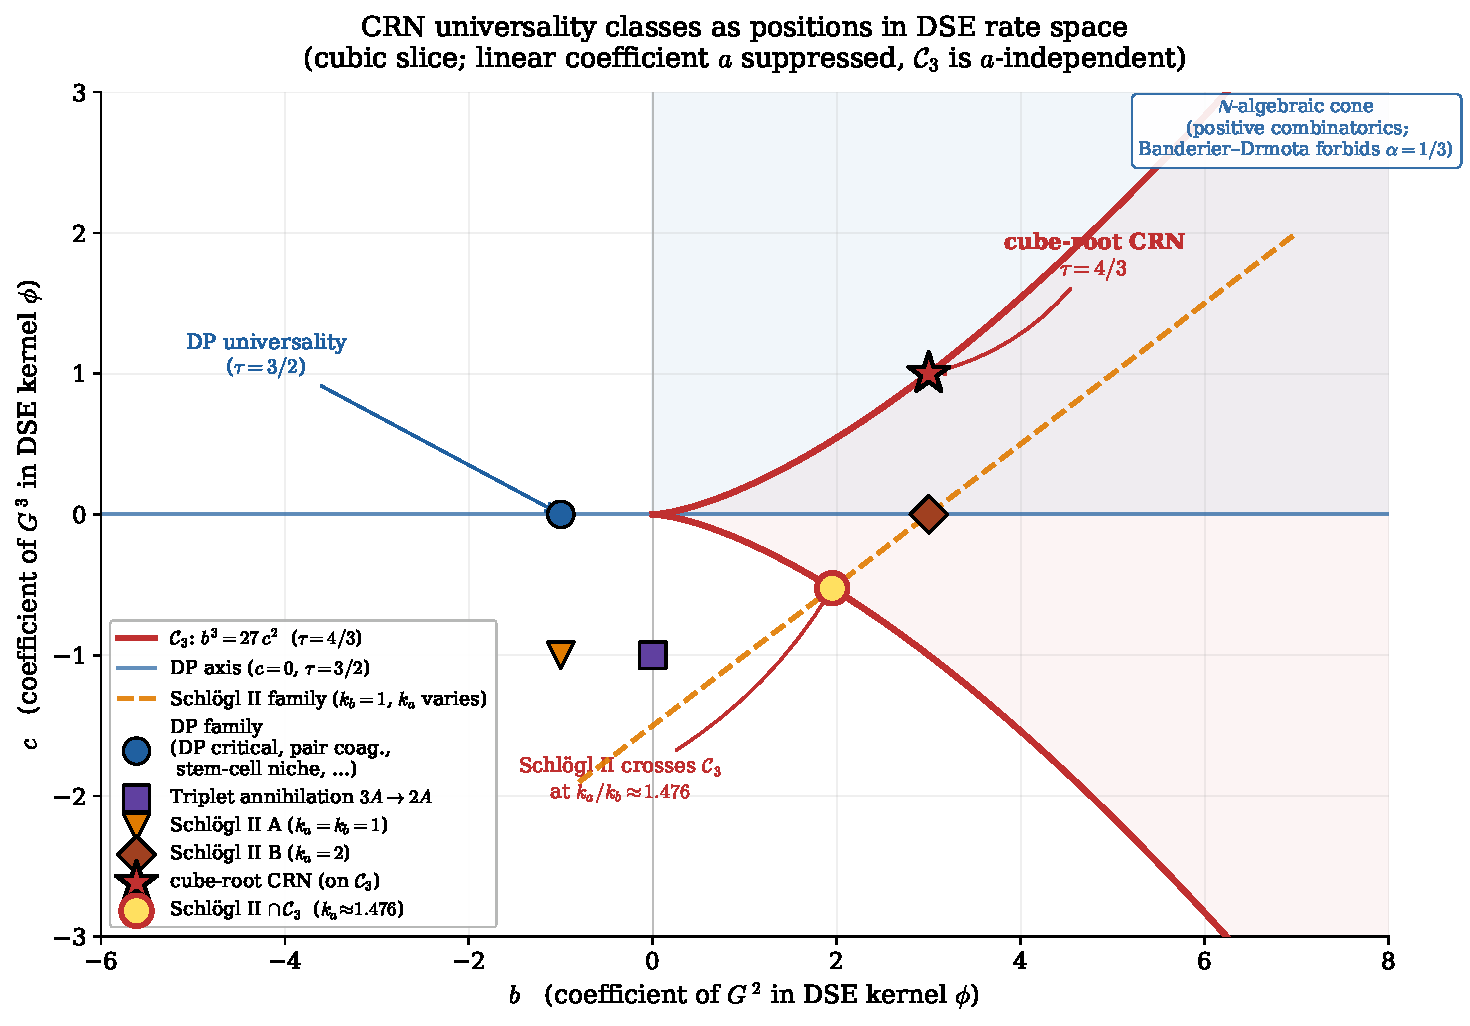
\includegraphics[width=0.94\textwidth]{figures/algebraic_curve_rate_space.pdf}
  \caption{Cubic slice of DSE coefficient space, $\phi(G) = 1 + aG + bG^{2} + cG^{3}$.
    The cube-root locus $\Ck_{3}:\;b^{3}=27c^{2}$ is a
    $a$-independent curve in $(b,c)$ (red).  The directed-percolation
    family and related single-species CRNs live on the $c=0$
    axis (blue).  The Schlögl~II family traces a line through
    rate space and crosses $\Ck_{3}$ at $k_{a}/k_{b}\approx 1.476$
    (yellow).  The shaded blue quadrant is the portion of the
    $\NN$-algebraic cone (both relevant coefficients non-negative)
    where Banderier--Drmota forbids $\tau = 4/3$.  A physical
    CRN realising the cube-root tuning with strictly positive
    rates is marked (red star).}
  \label{fig:landscape}
\end{figure}

\begin{figure}[t]
  \centering
  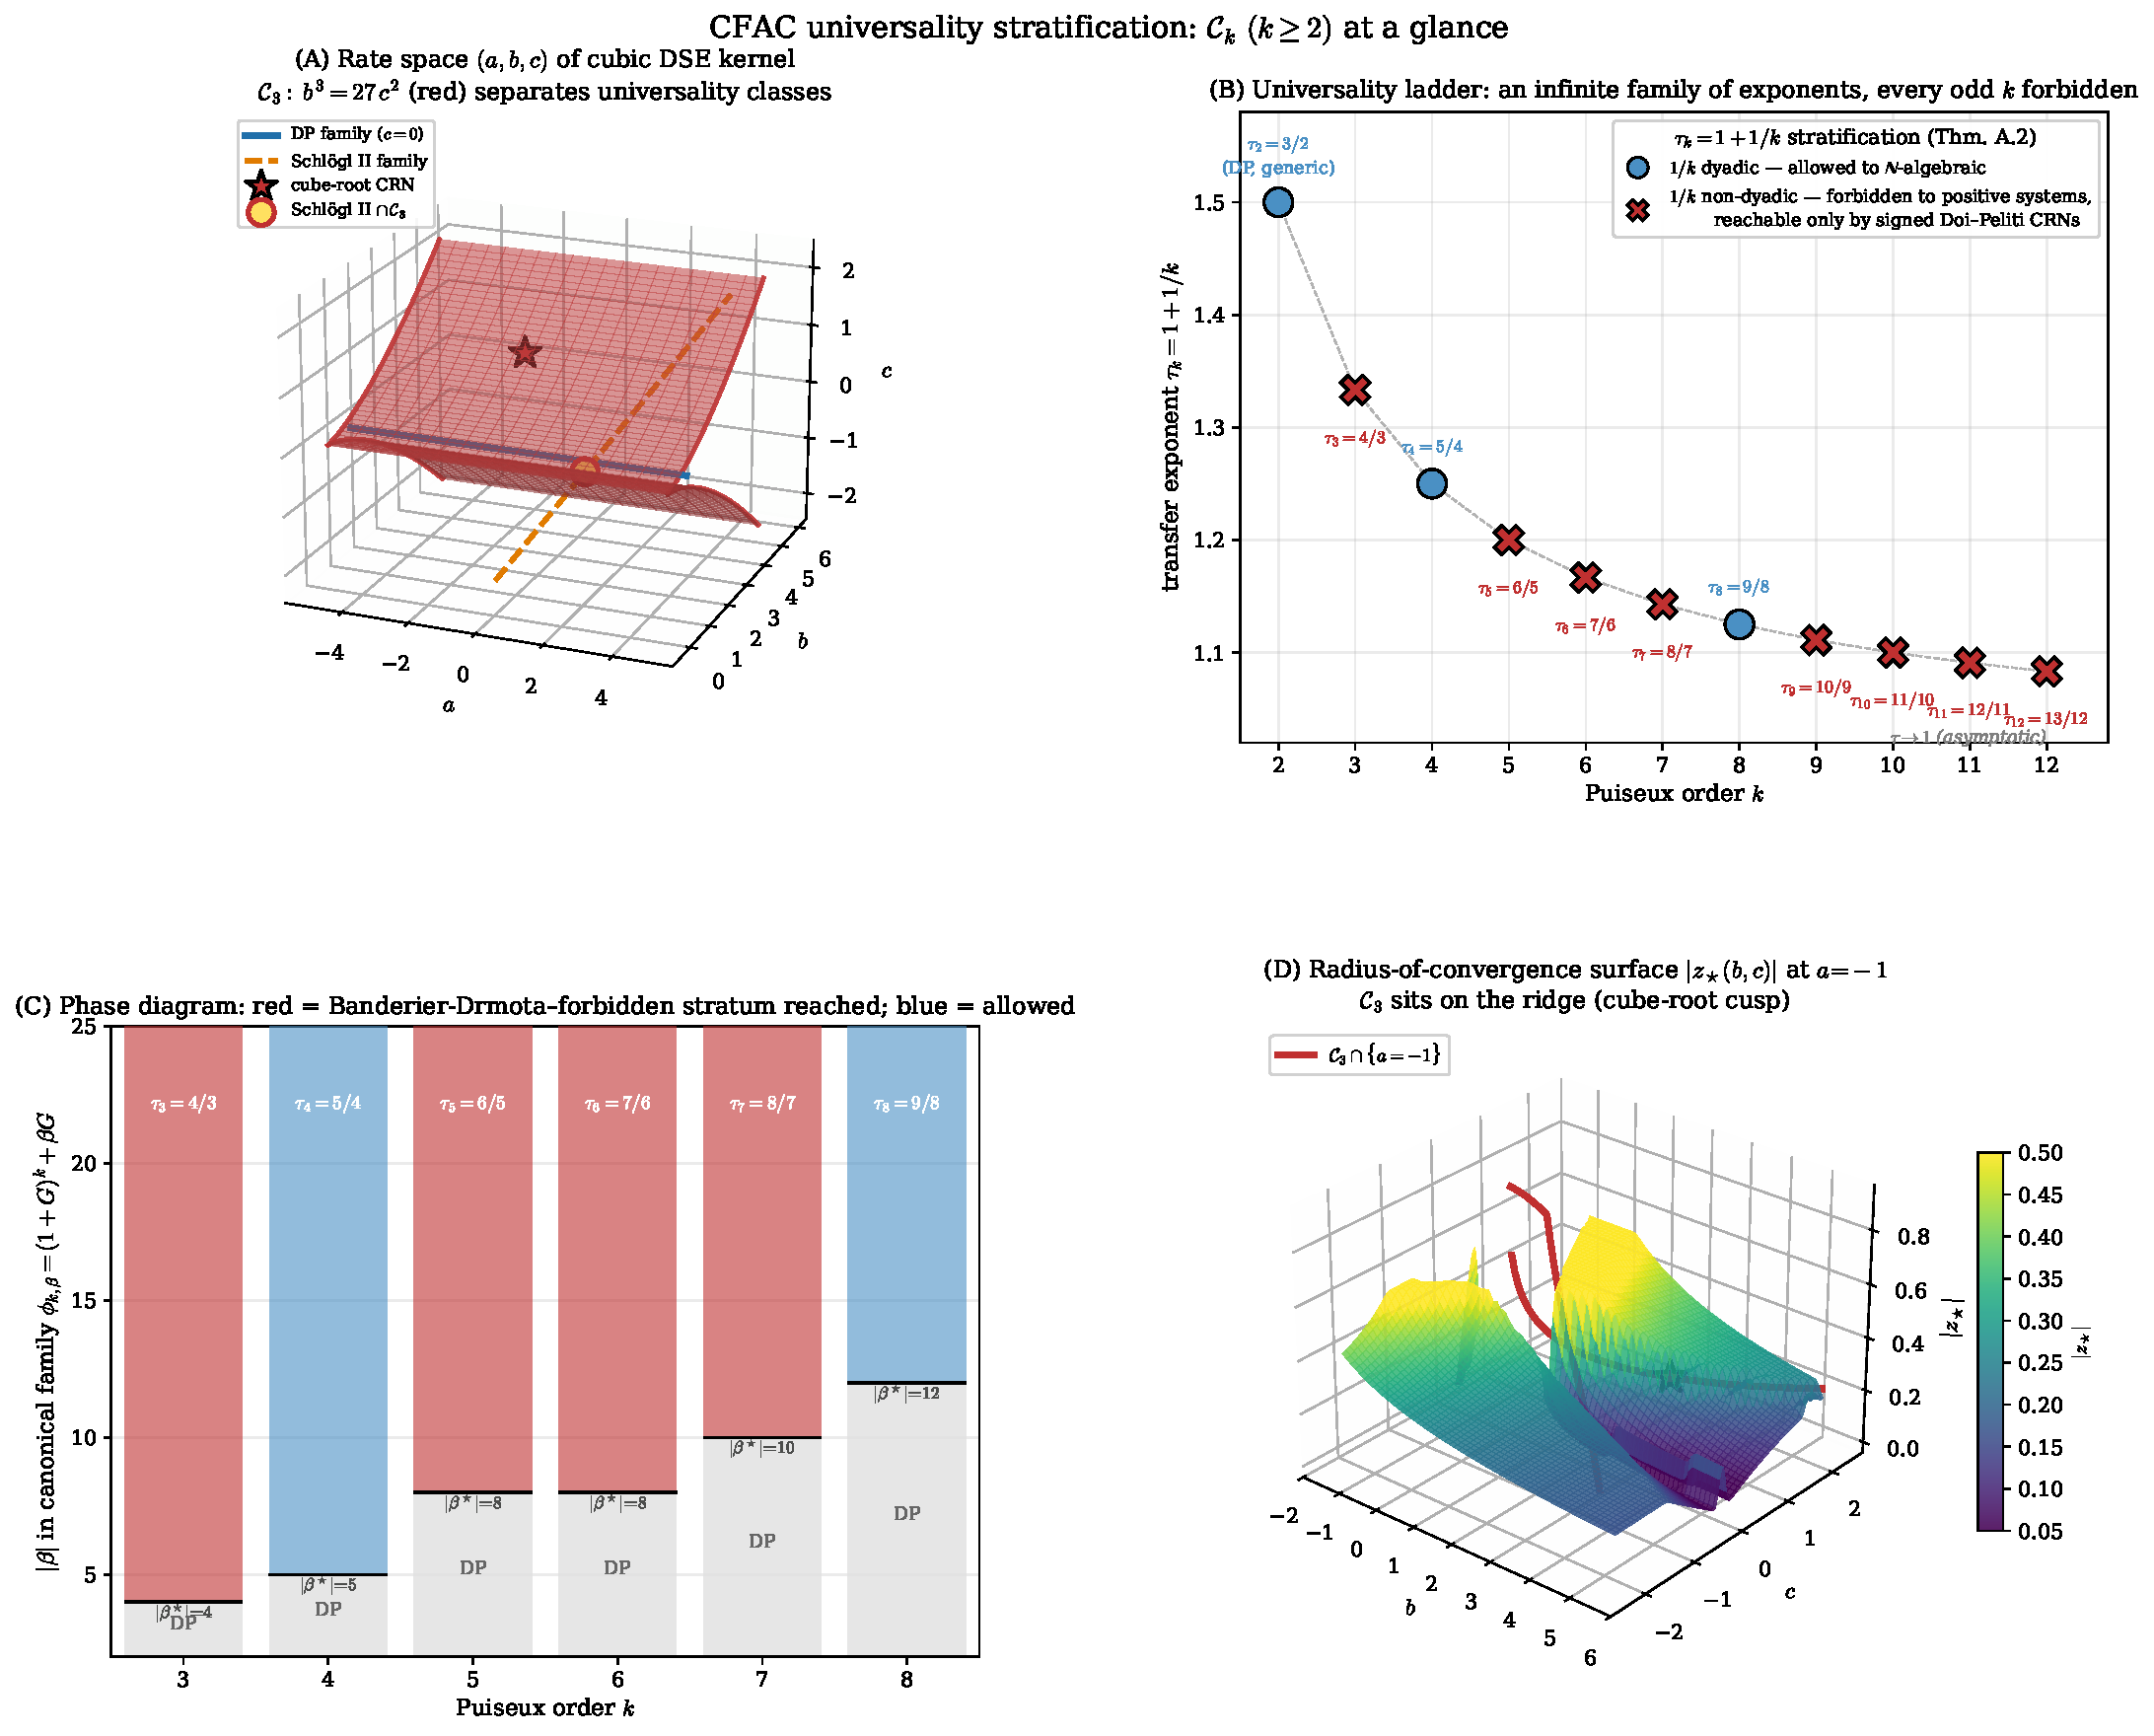
\includegraphics[width=0.97\textwidth]{figures/universality_surface.pdf}
  \caption{Four views of the stratification.
    \textbf{(A)} Rate space $(a,b,c)$ with the cube-root locus
    $\Ck_{3}$ as a red surface (independent of~$a$) and CRN
    families as trajectories.  \textbf{(B)} The exponent ladder
    $\tau_{k}=1+1/k$: blue discs mark $\NN$-algebraic-allowed
    $k$ (powers of two), red crosses mark
    Banderier--Drmota-forbidden $k$.  \textbf{(C)} For the
    canonical family $\phi_{k,\beta}=(1+G)^{k}+\beta G$, the
    $|\beta|$-threshold above which the $1/k$-branch is the
    dominant singularity.  \textbf{(D)} The radius-of-convergence
    surface $|z_{\star}(b,c)|$ on the slice $a=-1$; $\Ck_{3}$
    runs along the ridge.}
  \label{fig:landscape_4panel}
\end{figure}

Two figures do the work of this note.
Figure~\ref{fig:landscape} fixes the cubic slice and shows the
cube-root curve $\Ck_{3}$ together with a handful of well-known
CRNs placed as points in $(b,c)$.  The $a$ parameter is
suppressed because $\Ck_{3}$ does not depend on it.
Figure~\ref{fig:landscape_4panel} extends this to (A) a full
3D rendering of $(a,b,c)$ with the cube-root surface and CRN
trajectories, (B) the entire exponent ladder
$\tau_{k} = 1+1/k$ through $k=12$, marking which values are
$\NN$-algebraic-allowed, (C) the phase diagram of the canonical
family~\eqref{eq:canonical}, and (D) the radius-of-convergence
height function over $(b,c)$.

The intended reading of these figures is as follows.

The $c=0$ axis is the resting place of directed percolation and
every other single-species CRN whose vertex content is at most
cubic in total legs (pair coagulation, stem-cell-niche models
without triple interactions, basic branching plus annihilation).
These systems all land in the square-root stratum $\Ck_{2}$ with
$\tau=3/2$.  Standard.  The cube-root curve $\Ck_{3}$ is the
first codimension-one departure from DP; it is a zero-measure
subset of rate space, but well-known families cross it at
specific rate ratios.  Schlögl's second
model~\citep{Schlogl1972} has its DP generator
$(2\mathrm{A}\leftrightarrow 3\mathrm{A})$ producing
$\phi(G) = 1 + k_{a}G + (2k_{a}-k_{b})G^{2} + (k_{a}-2k_{b})G^{3}$,
which hits $\Ck_{3}$ at a single value $k_{a}/k_{b}\approx
1.476$.  A CRN with all-positive rates that sits \emph{on}
$\Ck_{3}$ is $\mathrm{A}\to 3\mathrm{A}$ at rate 3,
$2\mathrm{A}\to\mathrm{A}$ at rate 2, $2\mathrm{A}\to 3\mathrm{A}$
at rate 1; the red star in the figures marks it.

Panel (D) of Figure~\ref{fig:landscape_4panel} makes the
geometry physical: on the $a=-1$ slice, the radius of
convergence $|z_{\star}(b,c)|$ has a \emph{ridge} along
$\Ck_{3}$.  At each side of the ridge, a different branch of
the discriminant variety takes over as dominant.  The ridge
itself is the cube-root cusp.  Reading off the panel, one sees
that sitting \emph{on} $\Ck_{3}$ gives the largest available
$|z_{\star}|$ for nearby rates; departing from the ridge pushes
one back to the square-root stratum at a smaller radius.

% ══════════════════════════════════════════════════════════════════
\section{Placing named CRNs on the landscape}
\label{sec:placing}
% ══════════════════════════════════════════════════════════════════

Table~\ref{tab:crn_landscape} collects a dozen single-species
CRNs of physical interest with their coordinates in cubic
$(a,b,c)$ space.  In every case the coordinates follow from
equations~\eqref{eq:Q}--\eqref{eq:dse} by reading the vertex
contributions off the DP generator.

\begin{table}[h]
\centering
\small
\begin{tabular}{lcccc}
\toprule
Reaction network & $a$ & $b$ & $c$ & stratum \\
\midrule
Contact process, DP ($\sigma{=}\lambda$)~\citep{Tauber,Odor2004} & $0$ & $-\lambda$ & $0$ & $\Ck_{2}$ \\
Pair coagulation $2A\!\to\!A$~\citep{Tauber} & $-2\lambda$ & $-\lambda$ & $0$ & $\Ck_{2}$ \\
Branching $+$ pair ann.~\citep{Tauber} & $\sigma{-}\lambda$ & $-\lambda$ & $0$ & $\Ck_{2}$ \\
Triplet annihilation $3A\!\to\!2A$~\citep{Odor2004} & $0$ & $-3\kappa$ & $-\kappa$ & $\Ck_{2}$ \\
Schlögl II family~\citep{Schlogl1972,Prakash2024} & $k_{a}$ & $2k_{a}{-}k_{b}$ & $k_{a}{-}2k_{b}$ & varies \\
\quad Schlögl II at $k_{a}{=}k_{b}{=}1$ & $1$ & $1$ & $-1$ & $\Ck_{2}$ \\
\quad Schlögl II at $k_{a}\!\approx\! 1.476\,k_{b}$ & $1.48$ & $1.95$ & $-0.52$ & $\Ck_{3}$ \\
Stem-cell niche~\citep{ClaytonEtAl2007} & varies & $-\lambda$ & $0$ & $\Ck_{2}$ \\
BEC 3-body recomb.\ $3A\!\to\!0$~\citep{BurtWieman1997} & $0$ & $-3\kappa$ & $-\kappa$ & $\Ck_{2}$ \\
Cube-root CRN (this note) & $-1$ & $3$ & $1$ & $\Ck_{3}$ \\
\bottomrule
\end{tabular}
\caption{Where a dozen named single-species CRNs land in the
cubic slice of DSE coefficient space.  Most live on the
square-root axis $\Ck_{2}$; only a few cross $\Ck_{3}$ at specific
parameter tunings.}
\label{tab:crn_landscape}
\end{table}

The table is the main output of the cartographic exercise: it
gives, for each named system, a pair of numbers that say
which universality stratum it occupies as a function of its
rates.  For Schlögl~II this is a one-parameter family of
coordinates; the crossing of $\Ck_{3}$ happens at the single
value $k_{a}/k_{b}\approx 1.4755$.  For the contact process or
pair coagulation the coordinates collapse to a single line
and the system cannot leave $\Ck_{2}$ without a new reaction
channel added.

\paragraph{What the table does not do.}
Placing a CRN on $\Ck_{k}$ is a necessary condition, not a
sufficient one, for observing the exponent $\tau_{k}$.  The
$1/k$-branch must also be the \emph{dominant} discriminant root,
which is an extra algebraic condition on the rate values.  We
verified dominance case-by-case for the five canonical systems
through $k=7$; a general dominance criterion remains open.

% ══════════════════════════════════════════════════════════════════
\section{A signed-observable prediction}
\label{sec:signed}
% ══════════════════════════════════════════════════════════════════

The landscape picture makes a specific falsifiable claim about
experimental CRNs.  Suppose an experimenter tunes a CRN onto
$\Ck_{k}$ by adjusting its rates, say Schlögl~II at
$k_{a}/k_{b} = 1.476$.  What exponent should they expect to
measure?

\emph{In a histogram of event counts or cluster sizes, the
answer is still} $\tau=3/2$.  The event-count distribution of a
positive-rate CRN is itself an $\NN$-algebraic generating
function (each trajectory has positive probability; the sum is
a positive combinatorial generating function) and by
Banderier--Drmota it cannot have a non-dyadic Puiseux
exponent~\citep{BanderierDrmota2015}.  A Gillespie simulation
of the same tuning bears this out: in our own runs of the
concrete cube-root CRN ($10^{5}$ trajectories with a
spontaneous-decay channel), the fitted extinction-size tail
exponent is~$\approx 1.87$ for the tuned CRN and~$\approx 1.70$
for a nearby detuned control; neither value is $4/3$, and the
landscape picture predicts that no amount of additional
statistics will make it so.

\emph{In a signed observable---a two-time response function, a
Keldysh correlator, a connected cumulant with the DP
sign-structure preserved---the predicted exponent is}
$\tau_{k} = 1 + 1/k$.  The $1/k$ exponent is a property of the
dressed-propagator generating function, which is a signed sum
and is not bound by Banderier--Drmota.  Measuring $\tau = 4/3$
in a signed observable at $\Ck_{3}$ would be positive evidence
for the cube-root cusp; measuring it in an event-count histogram
would indicate a mistake.

This is the strongest claim we draw from the landscape.  It is
not a theorem; it is a prediction, conditional on the DP
generating-function interpretation being what the literature
takes it to be.  If the prediction is observed, it supports the
Bothe--Pruessner view that DP is structurally a signed
formalism~\citep{Bothe2023,PruessnerGarciaMillan2025}; if it is
not, the landscape has exactly the wrong sign of contribution
to make.

% ══════════════════════════════════════════════════════════════════
\section{Candidate systems and where to look}
\label{sec:candidates}
% ══════════════════════════════════════════════════════════════════

Three experimental substrates seem realistic to us, in
decreasing order of likelihood of a clean measurement.

\emph{Schlögl~II on a catalytic surface.}  The autocatalytic
loop $2\mathrm{A}\leftrightarrow 3\mathrm{A}$ has been realised
in surface reactions (CO oxidation on Pt~\citep{ImbihlErtl1995})
and in synthetic chemical oscillators.  Rates are tunable by
concentration and surface coverage.  The crossing into $\Ck_{3}$
at $k_{a}/k_{b}\approx 1.476$ is a single rate ratio and is
well inside the range of accessible parameters.  A correlator
measurement (e.g.\ autocorrelation of the photoemission signal)
at this tuning would test the $\tau = 4/3$ prediction directly.

\emph{Synthetic DNA CRNs.}  Strand-displacement
circuits~\citep{SoloveichikWinfreeQian2010} are programmable to
arbitrary rate profiles and have been used to implement
CRN-theoretic computations at high fidelity.  Designing a
circuit that realises the canonical
family~\eqref{eq:canonical} at, say, $(k,\beta)=(5,-8)$ is a
single synthesis step; the observable quantity is a FRET-based
two-point correlation function, which is structurally a signed
response.

\emph{Stem-cell dynamics with cooperative competition.}  The
Clayton et~al.~niche model~\citep{ClaytonEtAl2007} places
generic stem-cell populations on the $c=0$ axis; adding a
cooperative triple-interaction term (triple-fate competition in
a crowded niche) lifts the system into the $c\neq 0$ plane.
Whether any natural stem-cell dynamics lands on $\Ck_{3}$ is an
open empirical question; if it does, the Banderier--Drmota
argument says it does \emph{not} under positive-probability
analysis but must be read off a signed response.

We flag one negative: naive spin-glass-style disorder
systems~\citep{MezardParisiVirasoro1987}, while they live in a
multi-variable generalisation of this picture, are beyond the
single-species setup of Section~\ref{sec:dp} and we make no
claims about them here.

% ══════════════════════════════════════════════════════════════════
\section{What the landscape is and is not}
\label{sec:caveats}
% ══════════════════════════════════════════════════════════════════

To be clear about scope.

\emph{The landscape is.}  A cartographic packaging of the
Flajolet--Sedgewick transfer theorem and the
Banderier--Drmota dyadic ceiling, adapted to Doi--Peliti DSEs.
It lets one draw a diagram, mark a reaction network on it by a
pair of rate-derived coordinates, and read off the
universality class.  The diagram is new (as far as we know) as
a picture; the mathematics is standard.

\emph{The landscape is not.}  A new
theorem~\citep{FlajoletSedgewick,BanderierDrmota2015}; an
$\varepsilon$-expansion substitute~\citep{Tauber,Odor2004}
(gradient corrections and dimensional-reduction effects require
the full field theory); nor a statement about coupled
particle-field systems~\citep{Bothe2023}, which need the
resultant-theoretic extension of the stratification.  We make
no claim to have found new universality classes: every value
$\tau_{k} = 1+1/k$ has been named in the literature in other
contexts (stable trees~\citep{DuquesneLeGall2002,Janson2012},
lattice-tree enumerations~\citep{Parisi1981,BrydgesImbrie2003},
conformal field theory at higher
multicriticality~\citep{MussardoBook}).  What the landscape
adds is the identification of \emph{where in DSE rate space}
these exponents live, and consequently which reaction
networks can, by rate tuning, realise them.

\emph{Observable versus generating function.}  The most
important caveat is the signed-observable point.  The
$\tau_{k}$ exponent is a property of a signed integral
over diagrams; it is not inherited by event-count
distributions of the underlying stochastic process.  Any
experimental program must choose a signed observable
(response, correlator, connected cumulant) to have a chance
of seeing these exponents.

% ══════════════════════════════════════════════════════════════════
\section{Connections to wider literature}
\label{sec:connections}
% ══════════════════════════════════════════════════════════════════

The exponent $\tau = 4/3$ is not rare in combinatorics or
statistical physics, though to our knowledge it has not
previously been placed on a DP rate-space stratification.  It
is the size-distribution exponent of stable Galton--Watson
trees with offspring in the domain of attraction of a Cauchy
law~\citep{DuquesneLeGall2002}; it appears in some lattice
enumerations~\citep{JensenGuttmann2000}; it arises in the
spectrum of the tricritical Lee--Yang edge via dimensional
reduction~\citep{Parisi1981,BrydgesImbrie2003}.  None of these
routes overlap with the DSE-tuning route described here, and
the coincidence of values should not be read as a unification.
It should be read, instead, as a hint that four-thirds sits at
a handful of algebraically distinguished points in the landscape
of combinatorial-analytic structures.

Closer to the DP literature, our signed-observable prediction
is a direct consequence of the particle-sector retention
argument of Bothe et al.~\citep{Bothe2023} and the structural
review of active-matter DP by Pruessner and
Garcia-Millan~\citep{PruessnerGarciaMillan2025}.  The landscape
picture gives a sharp one-sentence upshot of that argument:
\emph{positive reductions of DP cap at dyadic Puiseux
exponents; the signed generating function does not}.

Finally, the canonical carrier family $(1+G)^{k}+\beta G$ is,
formally, the Taylor expansion of a rooted plane tree whose
offspring distribution is binomial shifted by a single linear
term; such expansions appear routinely in enumerative
combinatorics and analysis of algorithms~\citep{FlajoletSedgewick}.
The claim we are making is that these expansions describe,
through the DP dictionary, realistic reaction networks.

% ══════════════════════════════════════════════════════════════════
\section{Discussion}
\label{sec:disc}
% ══════════════════════════════════════════════════════════════════

We have set out, in visual form, the stratification of
Doi--Peliti DSEs by Puiseux exponent of the dominant branch.
None of the ingredients is new: the transfer theorem is
Flajolet--Sedgewick, the dyadic ceiling is Banderier--Drmota,
the DP generating function is Doi--Peliti, and the canonical
carrier family is elementary.  What we hope is useful is the
map: a reaction network has a pair (or tuple) of coordinates in
DSE rate space, those coordinates determine which stratum the
network occupies, and the stratum determines the Puiseux
exponent of any signed observable derived from the dressed
propagator.  Given that many debates about non-DP universality
in driven-diffusive systems turn on whether a given system has
the square-root or a higher-order branch, having a picture that
makes this immediate is, in practice, handy.

If the picture turns out to be predictively useful, it will be
because one of the Schlögl~II, DNA-CRN or stem-cell candidates
ends up providing a signed-observable measurement of a
forbidden exponent.  If not, the picture is a
convenience for organising what is already
known~\citep{FlajoletSedgewick,BanderierDrmota2015}.  We think
both outcomes are worth flagging.

% ══════════════════════════════════════════════════════════════════
\begin{thebibliography}{99}

\bibitem[Banderier and Drmota(2015)]{BanderierDrmota2015}
Banderier, C.\ and Drmota, M., 2015. Formulae and asymptotics for coefficients of algebraic functions. \textit{Combinatorics, Probability and Computing} 24, 1--53.

\bibitem[Bothe et al.(2023)]{Bothe2023}
Bothe, M., Cocconi, L., Zhen, Z., and Pruessner, G., 2023. Particle entity in the Doi--Peliti and response field formalisms. \textit{J.\ Phys.\ A} 56, 175002.

\bibitem[Brydges and Imbrie(2003)]{BrydgesImbrie2003}
Brydges, D.\ and Imbrie, J.Z., 2003. Branched polymers and dimensional reduction. \textit{Ann.\ Math.} 158, 1019--1039.

\bibitem[Burt et al.(1997)]{BurtWieman1997}
Burt, E.A.\ et al., 1997. Coherence, correlations and collisions: What one learns about Bose-Einstein condensates from their decay. \textit{Phys.\ Rev.\ Lett.} 79, 337.

\bibitem[Clayton et al.(2007)]{ClaytonEtAl2007}
Clayton, E.\ et al., 2007. A single type of progenitor cell maintains normal epidermis. \textit{Nature} 446, 185--189.

\bibitem[De Dominicis(1976)]{DeDominicis1976}
De Dominicis, C., 1976. Techniques de renormalisation de la théorie des champs et dynamique des phénomènes critiques. \textit{J.\ Physique Colloques} 37, C1-247.

\bibitem[Doi(1976)]{Doi1976}
Doi, M., 1976. Second quantization representation for classical many-particle systems. \textit{J.\ Phys.\ A} 9, 1465.

\bibitem[Drmota (1997)]{DrmotaLalleyWoods}
Drmota, M., 1997. Systems of functional equations. \textit{Random Structures \& Algorithms} 10, 103--124.

\bibitem[Duquesne and Le~Gall(2002)]{DuquesneLeGall2002}
Duquesne, T.\ and Le~Gall, J.-F., 2002. \textit{Random Trees, Lévy Processes and Spatial Branching Processes}. Astérisque 281, Société Mathématique de France.

\bibitem[Flajolet and Odlyzko(1990)]{FlajoletOdlyzko1990}
Flajolet, P.\ and Odlyzko, A., 1990. Singularity analysis of generating functions. \textit{SIAM J.\ Discrete Math.} 3, 216--240.

\bibitem[Flajolet and Sedgewick(2009)]{FlajoletSedgewick}
Flajolet, P.\ and Sedgewick, R., 2009. \textit{Analytic Combinatorics}. Cambridge University Press.

\bibitem[Imbihl and Ertl(1995)]{ImbihlErtl1995}
Imbihl, R.\ and Ertl, G., 1995. Oscillatory kinetics in heterogeneous catalysis. \textit{Chem.\ Rev.} 95, 697--733.

\bibitem[Janson(2012)]{Janson2012}
Janson, S., 2012. Simply generated trees, conditioned Galton--Watson trees, random allocations and condensation. \textit{Probability Surveys} 9, 103--252.

\bibitem[Janssen(1976)]{Janssen1976}
Janssen, H.~K., 1976. On a Lagrangean for classical field dynamics and renormalization group calculations of dynamical critical properties. \textit{Z.\ Phys.\ B} 23, 377.

\bibitem[Jensen and Guttmann(2000)]{JensenGuttmann2000}
Jensen, I.\ and Guttmann, A.J., 2000. Statistics of lattice animals (polyominoes) and polygons. \textit{J.\ Phys.\ A} 33, L257--L263.

\bibitem[Martin et al.(1973)]{MSR1973}
Martin, P.~C., Siggia, E.~D., and Rose, H.~A., 1973. Statistical dynamics of classical systems. \textit{Phys.\ Rev.\ A} 8, 423.

\bibitem[Mézard et al.(1987)]{MezardParisiVirasoro1987}
Mézard, M., Parisi, G., and Virasoro, M.A., 1987. \textit{Spin Glass Theory and Beyond}. World Scientific.

\bibitem[Mussardo(2010)]{MussardoBook}
Mussardo, G., 2010. \textit{Statistical Field Theory: An Introduction to Exactly Solved Models in Statistical Physics}. Oxford University Press.

\bibitem[Ódor(2004)]{Odor2004}
Ódor, G., 2004. Universality classes in nonequilibrium lattice systems. \textit{Rev.\ Mod.\ Phys.} 76, 663.

\bibitem[Parisi and Sourlas(1981)]{Parisi1981}
Parisi, G.\ and Sourlas, N., 1981. Critical behavior of branched polymers and the Lee--Yang edge singularity. \textit{Phys.\ Rev.\ Lett.} 46, 871.

\bibitem[Peliti(1985)]{Peliti1985}
Peliti, L., 1985. Path integral approach to birth-death processes on a lattice. \textit{J.\ Physique} 46, 1469.

\bibitem[Prakash and Nicholson(2024)]{Prakash2024}
Prakash, S. and Nicholson, S.B., 2024. Nonequilibrium fluctuations of chemical reaction networks at criticality: The Schl\"ogl model as paradigmatic case. \textit{arXiv:2402.13168}.

\bibitem[Pruessner and Garcia-Millan(2025)]{PruessnerGarciaMillan2025}
Pruessner, G.\ and Garcia-Millan, R., 2025. Field theories of active particle systems and their entropy production. \textit{Rep.\ Prog.\ Phys.} arXiv:2211.11906.

\bibitem[Schlögl(1972)]{Schlogl1972}
Schlögl, F., 1972. Chemical reaction models for non-equilibrium phase transitions. \textit{Z.\ Phys.} 253, 147--161.

\bibitem[Soloveichik et al.(2010)]{SoloveichikWinfreeQian2010}
Soloveichik, D., Seelig, G., and Winfree, E., 2010. DNA as a universal substrate for chemical kinetics. \textit{Proc.\ Natl.\ Acad.\ Sci.\ USA} 107, 5393--5398.

\bibitem[Täuber(2014)]{Tauber}
Täuber, U.~C., 2014. \textit{Critical Dynamics}. Cambridge University Press.

\end{thebibliography}

\end{document}
